\documentclass[12pt]{article}
\usepackage[spanish, es-tabla]{babel} % hace que, entre otras, el rompimiento de palabras se haga de acuerdo a las reglas del español
\selectlanguage{spanish}
\usepackage[utf8]{inputenc} % Incluye caracteres con tilde

\usepackage{pdfpages}
\usepackage{amsmath}
\usepackage{dsfont}

\usepackage{graphicx}   % permite insertar figuras
\usepackage{fancyhdr}   % para encabezado y pie de pagina
\usepackage{listings}   % para escribir código
\lstset{ % para configurar parámetros generales del código a mostrar en este documento
	commentstyle=\color{green},
	tabsize=4,
	numbers=left,
	literate={\ \ }{{\ }}1 % para fijar la tabulación
}	

%\usepackage{hyperref}   % crea links en el indice y notas al pie.
\usepackage{float}      % permite dejar las imagenes es una posición fija   
\usepackage[colorinlistoftodos]{todonotes} % permite agregar comentarios al documento.
\usepackage{mathtools}  % agrega funcionalidades nuevas a las fórmulas matemáticas.
\usepackage[font=footnotesize,labelfont=bf]{caption} % permite cambiar el tamaño de los textos en las figuras. Puede ser scriptsize, footnotesize, small, normalsize, large, Large.

%\usepackage{anysize}   % Permite emplear cualquier medida de márgenes.
%\marginsize{3cm}{2cm}{3cm}{2cm} % Controla los márgenes {izquierda}{derecha}{arriba}{abajo}. 

\pagestyle{fancy}

\setlength{\headheight}{15.9pt} % configurar la altura del header

%\lhead{Introducción al trabajo de titulo}
\chead{CC6908}
\rhead{}%
\includegraphics[width=30pt]{../images/LogoDCC.png}}

\usepackage{enumerate}
\usepackage{amsfonts} % para letras que representan conj numericos (R,Z,N,....)

% se aumenta la profundidad de la enumeración
\setcounter{secnumdepth}{5}
\setcounter{tocdepth}{5}

    \usepackage{setspace} % para controlar el interlineado

    \newcommand{\anchoFirma}{1.5in}

    %\newcommand*{\firma}[6]{
        % 1° fila : líneas horizontales donde se firma
            %    \noindent\makebox[\anchoFirma]{\hrulefill}
        %        \hfill\makebox[\anchoFirma]{\hrulefill}
        %        \hfill\makebox[\anchoFirma]{\hrulefill}\newline
            % 2° fila: cargos
            %    \noindent\makebox[\anchoFirma][l]{Profesor Guía:}\hfill
            %    \noindent\makebox[\anchoFirma][l]{Profesor Co-Guía:}\hfill
            %    \noindent\makebox[\anchoFirma][l]{Profesor Integrante:}\hfill
            % 3° fila: nombres profes
            %    \noindent\makebox[\anchoFirma][l]{#1}\hfill
            %    \noindent\makebox[\anchoFirma][l]{#2}\hfill
            %    \noindent\makebox[\anchoFirma][l]{#3}\hfill
            %    \\[0.5in]
            % 4° fila: línea para firmar
            %    \noindent\makebox[\anchoFirma]{}
        %        \hfill\makebox[\anchoFirma]{\hrulefill}
        %        \hfill\makebox[\anchoFirma]{}\newline
            % 5° fila: cargo
            %    \noindent\makebox[\anchoFirma][l]{}\hfill
            %    \noindent\makebox[\anchoFirma][l]{Memorista:}\hfill
            %    \noindent\makebox[\anchoFirma][l]{}\hfill
            % 6° fila: nombre memorista
            %    \noindent\makebox[\anchoFirma][l]{}\hfill
            %    \noindent\makebox[\anchoFirma][l]{#4}\hfill
            %    \noindent\makebox[\anchoFirma][l]{}\hfill
            % 7° fila: mail
            %    \noindent\makebox[\anchoFirma][l]{}\hfill
            %    \noindent\makebox[\anchoFirma][l]{#5}\hfill
            %    \noindent\makebox[\anchoFirma][l]{}\hfill
            % 8° fila: celular
            %    \noindent\makebox[\anchoFirma][l]{}\hfill
            %    \noindent\makebox[\anchoFirma][l]{#6}\hfill
            %    \noindent\makebox[\anchoFirma][l]{}\hfil
            %}


            \newcommand*{\firma}[8]{
                \noindent\makebox[1.5in]{\hrulefill}
                \hfill\makebox[1.5in]{\hrulefill}
                \hfill\makebox[1.5in]{\hrulefill}
                \noindent\makebox[1.5in][l]{#1}\hfill
                    \noindent\makebox[1.5in][l]{#3}\hfill
                    \noindent\makebox[1.5in][l]{#5}\hfill
                    \noindent\makebox[1.5in][l]{#2}\hfill
                    \noindent\makebox[1.5in][l]{#4}\hfill
                    \noindent\makebox[1.5in][l]{#6}\hfill
                    \noindent\makebox[1.5in][l]{}\hfill
                    \noindent\makebox[1.5in][l]{}\hfill
                    \noindent\makebox[1.5in][l]{#7}\hfill
                    \noindent\makebox[1.5in][l]{}\hfill
                    \noindent\makebox[1.5in][l]{}\hfill
                    \noindent\makebox[1.5in][l]{#8}\hfill
            }



\begin{document}

\renewcommand{\tablename}{Tabla} % Cambia la palabra cuadro por Tabla cuando se introducen tablas
\renewcommand{\listtablename}{Índice de tablas} % Cambia titulo de indice de tabla
%================================================================================================================
\begin{titlepage}
\vspace{2cm}
\begin{center}
{\large
    UNIVERSIDAD DE CHILE
        \\[0.1cm]
        Facultad de Ciencias Físicas y Matemáticas
        \\[0.1cm]
        Departamento de ciencias de la computación
        \\[0.1cm]
        CC6908 Introducción al trabajo de titulo
        \\[0.1cm]
}
\end{center}
% Imagen de la portada
\begin{figure}[h] %[h] para here [b] para bottom [t] para top
\makebox[\textwidth]{
\includegraphics[width=250pt]{../images/LogoFCFM.jpg}}
\end{figure}
\begin{center}
{\bf \huge \it Visualización de estructuras espaciales de desplazamiento a partir de datos de transporte público}
\\[1.0cm]
\today
\\[2.2cm]
\firma{Profesor Guía}{Marcela Munizaga}
{Profesor Co-guía}{Benjamín Bustos}
{Memorista}{Felipe A. Hernández G.} 
{fhernand@dcc.uchile.cl}{90977379}
\end{center}

\begin{center}
%Semestre: 02/2014\\
        %{\large \sc {\large Santiago de Chile}}
        \end{center}
        \end{titlepage}

        \newpage
        %================================================================================================================
        %\section{Resumen ejecutivo}

        %Aquí va el resumen ejecutivo

        %\thispagestyle{empty} % para que no se numere esta pagina+

        %\newpage
        %================================================================================================================
        \tableofcontents   % Indice

        \listoftables 	 % Indice de tablas

        \listoffigures   % Indice de figuras

        \pagenumbering{roman} % las páginas correspondientes al índice serán enumeradas con números romanos
        \newpage

        \pagenumbering{arabic}


        \newpage
        %================================================================================================================
        \section{Introducción}

        %\linespread{1.7}\selectfont

        En los últimos años la utilización de tecnología en el transporte público ha ido en aumento debido a varios factores, mayor regulación, usuarios más exigentes, aumento en seguridad, etc. Lo anterior ha llevado al sistema público de transporte a implantar diversos dispositivos que permiten controlar los aspectos mas relevantes al momento de transportar una persona de un punto a otro.

        Dentro de las tecnologías más usadas podemos nombrar AVL (Automatic Vehicle Location), que permite conocer la posición geográfica de un vehículo en todo momento con un margen de error bajo y los sistemas AFC (Automated Fare Collection) que automatizan el proceso de pago, en particular, nos interesa el basado en tarjetas de pago, que albergan un chip que permite mantener un saldo para que sea utilizado al abordar un bus, esto implica la existencia (paralelamente) de dispositivos asociados a los buses o paraderos\footnote{Lugar físico donde un bus de transporte público se detiene para que personas ingresen y/o desciendan a el.} que permitan registrar el correcto descuento del valor asociado al pasaje, concepto que llamaremos validación.
% hablar de los APC (Automatic passenger counting)

    Transantiago\footnote{fue implementado a partir del año 2007.} es el sistema de transporte público de Santiago de Chile que implementa las tecnologías nombradas anteriormente, por lo que hoy en día se sabe que se realizan aproximadamente 6.000.000 de validaciones durante un día laboral\footnote{Lunes, martes, miércoles, jueves o viernes.}, lo que genera una cifra cercana a los 35.000.000 de transacciones a la semana (incluyendo sábado y domingo) con aproximadamente 3.000.000 de tarjetas de pago. Por otro lado, hay 80.000.000 de emisiones proveniente de la tecnología AVL del sistema. Al procesar estos datos en conjunto es posible identificar el paradero de origen, recorrido utilizado para desplazarse y el paradero de destino, este último requiere un procesamiento adicional basado en una metodología desarrollada por Munizaga y Palma (2012) \cite{Procesamiento_datos} que logra una identificación en el 80\% de las validaciones.

    La estructura espacial moderna de las ciudades ha sido formada, en gran medida, por avances en transporte y comunicaciones \cite{Forma_ciudad_moderna}. La forma en la cual se mueven los habitantes de una ciudad ha ido modificando la estructura de ésta, motivados por la transferencia de recursos como materiales, dinero, personas e información. Considerando una persona como un transportador de recursos de un área urbana a otra es que se identifican las siguientes estructuras espaciales urbanas \cite{Estructura_urbana}:

    \begin{itemize}
    \item Centros de flujo: Se refiere a las áreas que sirven para conectar otro par de áreas para transferencia de personas. Funcionan como puentes espaciales entre distintas áreas.
    \item Centros: Se refiere a áreas que concentran personas. Pueden diferir de los Centros de flujo, pero a menudo, son lo mismo.
    \item Bordes: Se refiere a límites socioeconómicos generados a partir de la agrupación de paraderos que divide la ciudad en pequeños barrios que llamamos comunidades.
    \end{itemize}

    %hablar a quien va dirigido la visualización. Personas de áreas que no se realacionan directamente con la computación. Gente de arquitectura y urbanismo.
    % mencionar que el objetivo de la visualización es comunicar información.

    Lo anterior se enmarca en la necesidad de comunicar esta información de manera sintética dado que comprende una gran cantidad de datos y además abarcará otros campos de investigación, como lo es la arquitectura o planificación urbana, por lo que es necesario transmitir datos de forma clara y concisa.

    De todo lo relatado podemos ver que hoy en día el sistema de transporte público de Santiago cuenta con una gran cantidad de datos pasivos por lo que existe una gran base de datos que mantiene un potencial de información que puede ayudar a identificar problemas de acceso a servicios básicos, además de tener la potencialidad de detectar otras necesidades. Sin embargo, las herramientas de procesamiento actuales no logran obtener toda la información que los datos proveen.

    Según lo anterior, el problema que se busca resolver en esta memoria es interesante de abordar debido a que ayudará a entender la estructura espacial de los viajes realizados por la población. Esto ayudará a:

    \begin{itemize}
    \item Mejorar las posibilidades de realizar actividades en el entorno de la zona de residencia.
    \item Disminución de la demanda en los Centros de flujo.
    \item Disminución en el tiempo requerido para trasladarse hasta el punto de interés para una comunidad determinada.
    \item Mejorar las condiciones de viaje de grupos vulnerables.
    \end{itemize}

Esta memoria creará las estructuras espaciales mencionadas anteriormente a partir de los datos de transporte público de Santiago de Chile y diseñará una aplicación para que puedan ser visualizadas, de manera de comunicar información existente en los millones de datos provistos y que las herramientas actuales de procesamiento no abarcan.

    % hablar de esto en la motivación
    %Para detectar estos elementos en la ciudad de Santiago haremos uso de los datos obtenidos de su  sistema de transporte público utilizando para ello el análisis de redes (grafos) y algoritmos de procesamiento de estructuras de grafos a gran escala como infomap, además de herramientas computacionales para diseñar una interfaz de visualización de los datos.

    %Hoy en día la capacidad de procesamiento de datos a nivel industrial está muy lejos de lograr los que tienen los centros más avanzados, y a su vez, estos no tienen todo el procesamiento que desean. Según lo anterior es que debieron formularse diversos métodos de procesamiento que permiten acotar el tiempo en el cuál se puede extraer información. 

    \newpage
    %================================================================================================================
    \section{Motivación}
    %confort (tiene que ver con que la gente se pueda mover dentro del bus o metro)
%confiabilidad (variabilidad de intervalos)


    Como hemos dado a conocer, existe una gran fuente de datos con mucha información pero que actualmente encuentra sus dificultades en el procesamiento y la forma en que puede ser comunicada. Por lo que una solución a este problema puede abrir las puertas a nuevas preguntas y según esto, nuevas investigaciones.

    También es interesante académicamente debido a la masividad de los datos, ya que se deberá implementar una estrategia de procesamiento que permita manejar millones de registros y además realizar análisis sobre estos que permitan comunicar información por medio de la visualización.

    %\newpage
    %================================================================================================================
    \section{Objetivos}

    \subsection{Objetivo General}

    ``Diseñar una herramienta que permita identificar y visualizar estructuras espaciales de movimiento en la ciudad de Santiago de Chile utilizando datos pasivos y masivos de transporte público.''
    \subsection{Objetivos específicos}

    \begin{enumerate}
    \item Construir modelo de red para la ciudad de Santiago de Chile. %basado en los paraderos del transporte público.
    \item Identificar patrones de viaje, centros y centros de flujo.%puntos de alto flujo de pasada.
    \item Desarrollar una herramienta que permita visualizar las estructuras espaciales.
    \end{enumerate}

    \newpage
    %================================================================================================================
    \section{Metodología}

    %===================================================================
    % Arreglar aquí
    %====================================================================

    Esta metodología está basada en una investigación publicada en la \textit{International Journal of Geographical Information Science} \cite{Estructura_urbana}, por lo que los procedimientos ya han sido probados en otro contexto, reduciendo de esta forma posibles inconvenientes que puedan ocurrir a lo largo del desarrollo de esta memoria. 

    Los datos a utilizar se han definido como los producidos en una semana de calendario (lunes a domingo). Estos ya se encuentran procesados según la metodología diseñada por Munizaga y Palma (2012)\cite{Procesamiento_datos}, por lo que los datos corresponden a una tabla de una base de datos postgreSQL llamada \textit{tabla\_de\_etapas} donde cada fila representa una etapa de un viaje\footnote{un viaje puede tener una o más etapas.}. Según lo anterior la cantidad de datos a utilizar es de aproximadamente 35.000.000, que corresponde a la cantidad de etapas realizadas por el 80\% de las transacciones del sistema AFC\footnote{Automatic Fare Collection}.

    Dado lo anterior, el desarrollo de esta memoria considera la siguiente metodología de trabajo:

    \begin{enumerate}
    \item Investigación bibliográfica

    Se está realizando una recopilación y redacción de las ideas y estrategias más relevantes que aporten y justifiquen la base teórica de esta memoria.

    \item Estudio de los datos.

    Se realizará un estudio de los datos existentes para comprender concretamente las bases de datos requeridas.  

    \item Definición de estrategia de pre-procesamiento de datos.

    Se investigará sobre las estrategias de pre-procesamiento y elegirá la que mejor se adapte en base al estudio realizado en el item anterior. Dentro de esta etapa se llevará a cabo la normalización y selección de los datos para realizar los análisis.

    \item Construcción de la red de nodos.

    En esta etapa se realizará la construcción de un grafo dirigido con nodos a partir de los estudiados.

    \item Análisis de la red
    \begin{enumerate}
    \item Definición de propiedades básicas.

    Aquí asociaremos un atributo de las estructuras urbanas a cada propiedad matemática de un grafo a partir de las ideas obtenidas de la investigación bibliográfica.

    \item Definición de centralidades.
    \begin{enumerate}
    \item Centro de flujo.

    Se define el concepto de Centro de flujo en un grafo (\textit{centros de intermediación}) y se propone una fórmula para medirlo.

    \item Centro

    Aquí estudiaremos y definiremos la estrategia para detectar centros de la ciudad ocupando el algoritmo \textit{PageRank}.

    \end{enumerate}
    \item Estructura de comunidad.

    Para la detección de estructuras de comunidad se utilizará el software \textit{infomap}. 
    \end{enumerate}
    \item Análisis espacial
    \begin{enumerate}
    \item Interpolación espacial.

    Lo relevante de esta etapa es relacionar una zona geográfica a un paradero de bus de manera de poder particionar la ciudad.

    \item Cálculo estadístico.

    En esta etapa se realizará la asociación de las comunidades detectadas a las áreas geográficas establecidas en la interpolación espacial. El principal desafío aquí es corregir aquellas coordenadas que pertenecen a una comunidad en la red pero que no están geográficamente adyacentes al grupo principal que define la comunidad.

    \end{enumerate}
    \item Análisis de los resultados.

    Se estudiarán los resultados obtenidos.

    \item Definir visualizaciones y nivel de interactividad de cada una.

    A partir del punto anterior se definirán las visualizaciones a realizar y las posibles interacciones que puedan haber en cada una de ellas.

    \item Diseño de aplicación de visualización.

    Se desarrollará una aplicación que permita ver cada una de las implementaciones definidas en el punto anterior.

    \end{enumerate}

    Este trabajo será realizado a lo largo de 2 semestres (2014-2 y 2015-1) por lo que se dividirá de la siguiente forma:

    \begin{itemize}
    \item Semestre 2014-2
    \begin{enumerate}
    \item Investigación bibliográfica 
    \item Estudio de los datos
    \item Definición de estrategia de pre-procesamiento de datos
    % mencionar que esta parte se intentará completar. El compromiso es medio.
    \end{enumerate}
    \item Semestre 2015-1
    \begin{enumerate}\setcounter{enumi}{3}
    \item Construcción de la red de nodos
    \item Análisis de la red
    \item Análisis espacial
    \item Análisis de los resultados
    \item Definir visualizaciones y nivel de interactividad de cada una
    \item Diseño de aplicación de visualización
    \end{enumerate}
    \end{itemize}

    Es importante decir que el punto 3 se espera abordarlo de manera parcial, realizando un acercamiento durante este período para luego finalizarlo previo inicio del segundo y así poder lograr el desarrollo del resto.


    \newpage
    %================================================================================================================

    \section{Revisión de antecendentes}
    
    \subsection{Análisis de bibliografía}\label{sec:Analisis_bibliografia}
    
    Esta memoria se basa principalmente en la metodología propuesta por Cheng Zhong et al. (2014) \cite{Estructura_urbana}, la cual provee un método cuantitativo para la detección de \textbf{Centros de flujo}, \textbf{Centros} y \textbf{Bordes} pudiendo identificar estructuras urbanas a partir de datos pasivos de transporte público. Dentro de este mismo documento se establece una vinculación entre los centros de flujo, centros y bordes con fenómenos urbanos reales dado que utiliza un grafo generado a partir de datos obtenidos del comportamiento de la gente. Además permite aplicar nuevas técnicas para detección de bordes basadas en otras metodologías que puedan aparecer en el futuro, permitiendo la comparación entre ellas. Por lo tanto, la metodología allí expuesta es utilizada en esta memoria para la generación de las mismas estructuras pero para ser analizada con los datos locales de transporte público.
    
	\subsubsection{Redes espaciales} 
	
	Una red espacial se entiende como un grafo cuyos vértices y arcos representan objetos geométricos del mundo real. Los nodos tienen una posición relativa a un sistema de referencia específico y los arcos expresan la forma física en que interactúan entre ellos, entendiéndose esto último como la forma en que se puede llegar físicamente de uno a otro. El termino ``complejo"  se anexa al término de red espacial  cuando el grafo de esta red se caracteriza por tener propiedades estructurales que se relacionan con la accesibilidad de un nodo y su aporte dentro de la red. Estas propiedades tienen la particularidad de estar presentes en muchos problemas reales (Doursat 2005) \cite{doursat}.
		
	Hace algunos años atrás los análisis espaciales urbanos se limitaban a utilizar el diseño de las calles en términos de su topología urbana (Cardillo et al. 2006)\cite{cardillo}, lo que tiene la limitante de no considerar la accesibilidad asociada a una calle como una característica dependiente de los movimientos humanos existentes. Además, este tipo de análisis tiende a ignorar los flujos urbanos y a justificar espacios y su forma en función de las propiedades de la red.
	
	En los últimos años, los estudios sobre estás redes (Soh et al. 2010) \cite{soh} comenzaron a incorporar medidas de peso que reflejan los datos de movimientos urbanos como flujos sobre la red pero concentrado en el sistema de tránsito, no sobre los espacios urbanos asociados a estos .
	
	Además de los datos obtenidos a partir del transporte público han existido investigaciones basadas en otras fuentes de datos, como lo son los AVL basado en GPS (Rinzivillo
et al. 2012)\cite{rinzivillo} o conjuntos de datos telefónicos (Ratti et al. 2010)\cite{ratti}. En particular, el artículo de Cheng Zhong et al. (2014)  utiliza los datos generados a partir del uso de tarjetas inteligentes del transporte público de Singapur.
    
    
    \subsubsection{Construcción y representación de la red}\label{sec:contr_y_rep_red} 
	
	Formalmente definimos un grafo dirigido con pesos como $G=(N,L,W)$ que representa todas las etapas de viajes realizadas. $N$ denota los paraderos existentes, a éste se asocia el área o sector donde está ubicado, el conjunto $L$ denota los traslados entre dos paraderos o áreas, por lo que $L$ corresponde a un conjunto de pares ordenados de $N$, y el conjunto $W$ denota el volumen (cantidad) de traslados entre dos paraderos. Según lo anterior, $N$ son los nodos del grafo, $L$ representa los arcos y $W$ denota los pesos de cada arco en $L$.
	
	Por otro lado, Munizaga y Palma (2012) \cite{Procesamiento_datos} (explicado en la sección \ref{sec:Analisis_datos}) proponen una metodología para crear una \textit{matriz Origen-Destino}, generando la oportunidad de modelar la construcción teórica descrita en el párrafo anterior en sistemas donde solo se valida en un sentido, como lo es en el caso de Santiago de Chile.
	
	\subsubsection{Análisis complejo de la red}    

Este análisis se abarca desde 3 perspectivas: propiedades globales, información local asociada a \textit{centros} y \textit{centros de flujo}, y en la detección de comunidades. 

	\paragraph{Propiedades globales}

Las propiedades topológicas de un grafo pueden proveer importante información sobre las interacciones espaciales que se producen en el modelo real, según esto, se define lo siguiente

	\begin{itemize}
	
		\item El número $N$ de nodos indica cuantos paraderos o áreas son accesibles, y el número de arcos $J$ indica cuantos paraderos o áreas están directamente conectadas.
		\item El \textbf{grado} de cada nodo en la red indica cuantos paraderos o áreas están directamente conectadas desde una en particular, aquí podemos diferenciar entre \textbf{grado de salida} (cantidad de nodos que tienen traslados cuyo origen es ese paradero) y \textbf{grado de entrada} (cantidad de nodos que tienen como destino ese paradero).
		
		\item El \textbf{peso} de cada arco indica la intensidad (volumen) de traslados desde un paradero a otro.
		
		\item La \textbf{ruta más corta} se refiere al camino mínmo posible de un área a otra.
		
		\item \textbf{``clustering centrality''} es un índice que mide cuán cohesionados o cercanos están los nodos a otro en términos de su accesibilidad para compartir vecinos.

% the clustering centrality is an index that measures how ‘close’/‘cohesive’ the areas are to one another in terms of their accessibility to shared neighbors
		
		\item \textbf{Centralidad de cercanía} es un índice que evalúa cuan rápido viaja la información en un grafo. Se calcula para un nodo $i$ como $\frac{1}{lejania(i)}$, donde $lejania(i)=\frac{1}{|V|-1}\sum_{\forall j\not=i}\delta_{ij}$. Donde $\delta_{ij}$ es la distancia más corta de $i$ a $j$.
		
	\end{itemize}

Estas propiedades permiten descubrir los niveles de actividad que mantiene cada área de una ciudad y su participación en los flujos que se realizan.

	\paragraph{Centralidades}
	
	A las propiedades generales agregamos 2 tipos de centralidad adicionales, una es la \textit{centralidad de intermediación}, la que se usará para definir los \textbf{centros de flujo} y el segundo es el \textit{PageRank} que mide la accesibilidad en la red tomando en cuenta todos los vínculos, directos e indirectos, sus pesos y dirección. Este último indicador será útil para medir el grado en que cada nodo es un \textbf{centro}.
	
	La centralidad de intermediación es un indicador que mide cuán bien conectada está un área o paradero, formalmente se define para un nodo $k$ como el número de caminos más cortos que conecta dos áreas $i$ y $j$ en el grafo que pasan a través del nodo $k$, y se define como
	
$$
	C_{intermediacion}(k) = \sum_{ij} \frac{\delta_{ij} (k)}{\delta_{ij}}
$$

donde $\delta_{ij}(k)$ es el número de caminos más cortos entre $i$ y $j$ que pasan por $k$, mientras que $\delta_{ij}$ es el número total de caminos más cortos entre $i$ y $j$. Notar que $i$ y $j$ son distintos de $k$.
%En ciertos casos esta medida se normaliza dividiéndola por $N$ (cantidad de nodos) lo cual ellos no realizaron, utilizando la forma tal cual aparece en la definición. 

Por otro lado, \textit{PageRank} mide el rol de un nodo o área local en atraer flujos desde todos los nodos de la red. Esta medida puede ser vista como una representación genérica de las probabilidades de un peatón cualquiera de visitar un nodo cualquiera, en este sentido está relacionado con procesos de Markov de primer orden (Brin y Page 1998)\cite{markov}, que es la base de muchos procesos de interacción social, en este contexto  fue originalmente usado para extraer información acerca de las estructuras de los vínculos de Internet (Rosvall y Bergstrom 2008)\cite{Infomap}, muy similar al \textit{ranking de páginas de Google}. Según lo anterior de define la probabilidad $r_j$ de visitar el nodo $j$ como:

$$
	r_j = [(1-\rho)/N]+\rho\sum_i r_ip_{ij}
$$
% tiene toda la cara de ser probabilidades totales = 

% 1° termino = probabilidad de quedarme en el nodo j X la prob de elegir el nodo j.
% 2° termino = probabilidad de irme X la probabilidad de elegir algun otro nodo distinto de j

% probas totales r_j = P(de llegar a j | estoy en j)X P(estoy en j) + P(llegar a j | estoy en i)X P(estoy en i) 
%                    = (1-\rho)X(1/N) + \rhoXp_ijXr_i
%                       me quedo        sum (P(querer irme)X P(irme a j)X P(estar en i)) -> se repite para todos los nodos, luego se factoriza por \rho en la sumatoria

Donde $1-\rho$ puede ser visto como la probabilidad de que un caminante decida quedarse en el nodo $j$, y $p_{ij}$ como la probabilidad de escoger ir al nodo $j$ dado que estoy en el nodo $i$, este valor es proporcional al peso del arco de $i$ a $j$, en resumen

\begin{center}
$	p_{ij}=w_{ij}/\sum\limits_k w_{ik}$ , y $\sum\limits_j p_{ij}= 1$
\end{center}

%Dado que $r_j$ está definido en función de otros $r_k$ es necesario resolver un sistema matricial
%\todo{Explicar más.}

El parámetro $\rho$ es conocido como \textit{factor de amortiguación} y toma valores entre $0$ y $1$, en el estudio de Chen Zhong et al. (2014) fue fijado en $0.85$. Si $\rho=1$ entonces todos los nodos tienen una probabilidad positiva y luego, la matriz $\{p_{ij}\}$ tiene que estar fuertemente conectada.

	\paragraph{Estructura de comunidad}
	
	Los bordes a identificar sobre la superficie a analizar sirven para particionar la estructura espacial y así crear pequeños vecindarios a partir de ésta que denominamos comunidades. Estos son obtenidos a partir de la detección de una \textit{estructura de comunidad}, que se refiere a una \textbf{propiedad de un grafo que permite agrupar nodos de éste que están densamente conectados entre ellos en comparación con el resto de nodos del grafo}. Según lo anterior, los bordes son generados a partir de un descriptor de bordes que particiona la red en dos niveles donde los nodos forman módulos que llamamos comunidades y la división entre estos que llamamos bordes. Existen varias formas de generar comunidades pero una condición necesaria para este trabajo es la consideración de las variables  de \textbf{densidad} y \textbf{flujo de interacciones} al momento de crear éstas. Lo anterior basado en que estas dos variables deben ser mas fuertes dentro de una comunidad y que el volumen que está dentro de cada comunidad es mayor en comparación con el resto de la red.
	
	Para la generación de las comunidades se utiliza el framework \textit{mapEquation} basado en un procedimiento llamado \textit{infomap} desarrollado por Rosvall y Bergstrom el 2008 \cite{Infomap}. Lo anterior se justifica por Lancichinetti y Fortunato (2009)\cite{Comparar_generador_comunidad}, donde concluyen que es uno de los algoritmos que ha mostrado mejor rendimiento para la generación de comunidades y uno de los pocos adecuados para redes con peso y dirección. Otra característica relevante del algoritmo \textit{infomap} es que no solo considera la relación entre pares de nodos sino que también toma en cuenta los flujos presentes entre estos. 
	
	Para llevar a cabo lo anterior se utilizan flujos probabilisticos creados a partir de generaciones aleatoreas que simulan recorridos sobre el grafo y que asignan también probabilidades a cada nodo de ser visitado aleatoriamente (utilizando el algoritmo \textit{PageRank}), con el objetivo de modelar los comportamientos de flujo de un sistema real.
	% falta hablar que tienen la mínima entropía. Se justifica con la cita.
	
	En resumen, el algoritmo divide los nodos del grafo en módulos que son altamente estructurados, lo que implica que la entropía del grafo particionado es mínima (Rosvall y Bergstrom, 2008)\cite{Infomap}. Esta entropía total del sistema está dividida en la entropía de moverse entre los módulos más la entropía de moverse dentro de un módulo, las proporciones están relacionadas a la probabilidad de ocurrencia de cada uno. Por lo anterior, Rosvall y Bergstrom (2008) definen esta entropía como:
	$$
	\begin{rcases}
	Lg(M) &= H(P) + \sum\limits_{i=1}^m P_i H(p)_i \\
	      &= -p\sum\limits_{i=1}^m P_i log P_i -\sum\limits_{i=1}^m P_i\sum\limits_{k=1}^{M_i} \frac{P_k}{P_i}log\frac{P_k}{P_i}
	\end{rcases} , P_i = \sum_k p_k
	$$
% Es la entropía de moverse entre módulos más la entropía de moverse dentro de un módulo, normalizada(por ello la división de P_i)
	
donde $P_i$	es la probabilidad de ser visitada la comunidad $i$, $p$ es la probabilidad que un caminante cualquiera de cambiarse de modulo y $P_k$ es la probabilidad de visitar el nodo $k$. Además $M_i$ es la cantidad de nodos que contiene la comunidad $i$ y la división por $P_i$ que afecta a los $P_k$ cumple la función de normalizar.

La forma en que trabaja es primeramente asociando cada nodo al módulo que pertenece, donde en cada paso, se identifica que nodo se puede agregar a que módulo tal que la entropía general decrezca. Este proceso continua hasta que no se pueda reducir más la entropía, asegurando que con esa configuración se obtiene la partición más estructurada.

Es importante decir que $M_i$ es un módulo que contiene un conjunto de $k \in M_i$ nodos y que llega a ser estable (sin alteraciones) una vez que se obtiene la entropía mínima (Rosvall y Bergstrom, 2008). Luego, estas comunidades son mapeadas a sus respectivas ubicaciones geográficas.

Con lo anterior ya hecho, lo que restó por hacer fue transformar los conjuntos de puntos discretos obtenidos por \textit{PageRank} en regiones que particionan el espacio geográfico, para esto se realizó una interpolación espacial que considera el siguiente supuesto:

\begin{center}
	\textit{``Cada persona escoge el paradero de bus/metro más cercano a la posición en la que se encuentra"}
\end{center} 

Según lo anterior, Chen Zhong et al. (2014) propone aplicar una interpolación a cada zona geográfica cercana a un paradero de bus/metro. La variante de interpolación escogida corresponde a la \textit{Inverse Distance Weighting}(\textit{IDW}) lo que hace disminuir la influencia de un paradero de bus en función de la distancia. Estos pesos son definidos de la siguiente forma 

$$
	W_i(x,y) = 1/d_{ij} (x,y)^\lambda
$$

Donde $W_i(x,y)$ es el peso del paradero $i$ en las coordenadas $(x,y)$ que son los puntos vecinos más cercanos a $j$ y $d_{ij} (x,y)$ es la distancia a la coordenada $(x,y)$ desde el paradero $i$ hacia el paradero vecino más cercano $j$.

Una observación que se desprende de la fórmula es que los pesos están normalizados tal que su suma sea 1, es decir, $\sum_{\forall x,y} W_i (x,y)=1$ y $\lambda$ es un parámetro arbitrario que en este caso es $2$, lo que implica que sigue la ley del inverso al cuadrado.

Por último cada coordenada espacial fue asignada a una única comunidad, esto lo logran utilizando un  \textit{resumen estadístico}\footnote{Se entiende como la información dada por una rápida y simple descripción de los datos como la media, mediana, moda, rango y desviación estándar.}. El principal problema aquí fue tratar aquellas coordenadas que pertenecen a una comunidad en la red pero que no están geográficamente adyacentes al grupo principal que define la comunidad	, esto se origina porque el algoritmo de detección de comunidades no está restringido a lograr áreas geográficamente contiguas.

Aunque la investigación reporta que esto no ocurre muy a menudo, y que cuando sucede, es en los limites de las áreas que definen las comunidades y se da principalmente porque las personas que viven en esas áreas tienen diferentes preferencias de viajes.

Para solucionar el problema planteado se cuenta el número de puntos en las comunidades en conflicto y se computa el algoritmo \textit{PageRank}, esto provoca que las coordenadas en disputa sean asignadas a su comunidad más cercana geográficamente. En la práctica lo que se ocurre es un desplazamiento de los límites entre comunidades, de esta forma se obtiene una partición geográfica que abarca todo el espacio.
    
%	\subsubsection{Georeferenciación espacial}

%La georeferenciación espacial se refiere a un sistema de referencia que se utiliza para representar las ubicaciones de objetos o fenómenos  dentro de un marco geográfico común. Existen varios y cada uno queda definido por: punto de referencia, unidad de medición, entre otras \cite{argis}. 

%Existen dos tipos de sistemas de coordenadas que se utilizan ampliamente:

%\begin{description}
%	\item[latitud-longitud] son los denominados sistemas de coordenadas geográficas 
%	\item[proyectado] 
%\end{description}

%Los datos geoespaciales a diferencia de otros tipos de datos describen objetos o fenómenos con una ubicación específica en el mundo real. 

%\todo{Falta completar.}
%En esta sección se debe explicar que es la georeferenciación, para que sirve, su definición formal y que es lo que se puede lograr con ella.
    
	\subsubsection{Visualización de información}    
    
	En esta sección serán descritos algunos aspectos relevantes de la visualización de información con el fin de justificar teóricamente preguntas como: ¿que es la visualización? ¿que colores utilizar? ¿que tipo de visualización mostrar? ¿cuál es el objetivo de la visualización que estoy creando? entre otras. 
	
	Toda la información necesaria fue obtenida del libro \textit{Interactive Data Visualization: Foundations, Techniques, and Applications} \cite{libro_visualizacion}.

	\paragraph{¿Que es la visualización?} \hfill \\ % para que haga un salto de línea
	
	El concepto de visualización se define como la \textit{comunicación de información usando representaciones gráficas}. El beneficio de utilizar imágenes está dado por la riqueza de información que puede contener y el tiempo que requiere para ser procesada en vez de información en páginas con texto, esto ocurre debido a que la interpretación de imágenes es realizada en \textbf{paralelo} dentro del sistema perceptual mientras que la lectura es un proceso \textbf{secuencial}. Otra de las ventajas que tiene la visualización es su independencia del lenguaje, siendo más eficaz que un texto para un grupo de personas que hablan diferentes idiomas. 
	
	La importancia de esta forma de comunicación radica en que los seres humanos son seres visuales que usan la visión como uno de los sentidos claves para entender la información, según esto es que se justifica el hecho de que sea ocupada en muchos lugares en la toma de decisiones, y dado el incremento de datos presentes hoy en día en cada área del conocimiento, es que hay una creciente necesidad por herramientas y técnicas que ayuden a convertirlos en información útil. 
	
	%La visualización no es efectiva \textit{per se} sino que depende de varios factores su impacto. En 1999 Linda Elting demostró por medio de un experimento que la visualización afecta el proceso de decisión y que está muy relacionada con las preferencias y nivel de entrenamiento de los usuarios involucrados.
    
% sección 1.2.2 del libro
	\newpage
	\paragraph{Tipo de visualizaciones} \hfill \\
	
	La visualización a menudo ofrece distintos niveles de vistas de información. Dependiendo de que parte de la información existente es la relevante de ser mostrada tenemos
	
	\begin{description}		
		\item[Visualización cualitativa] En esta se distorsiona la imagen con el objetivo de destacar alguna cualidad en particular. Un ejemplo de esto se observa en la figura \ref{fig:metro}, que corresponde a la red de metro subterráneo de la ciudad de Tokio, en el se produce una distorsión de los puntos en donde se interceptan varias líneas para facilitar su interpretación. 
		
% Imagen de metro
\begin{figure}[h] %[h] para here [b] para bottom [t] para top
\makebox[\textwidth]{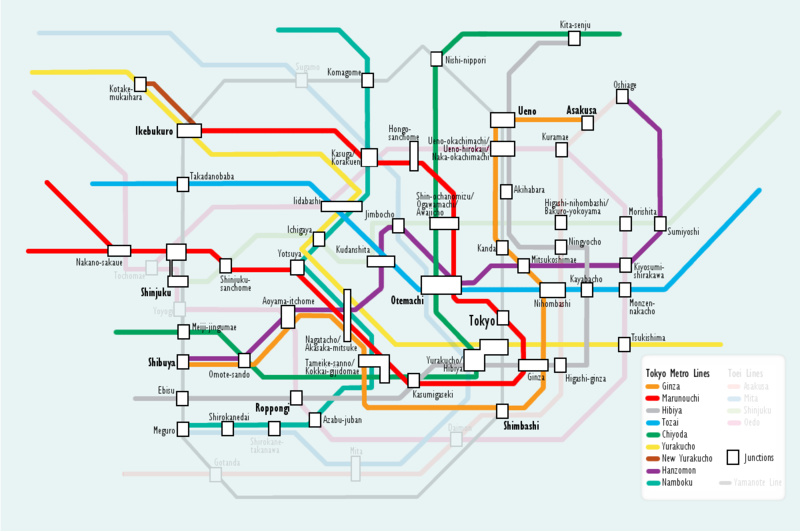
\includegraphics[width=350pt]{../images/metro_tokyo.png}}
\caption[Metro subterráneo de Tokio]{Metro subterráneo de Tokio. Representación cualitativa de las estaciones y las líneas que pasan por ella. (obtenida desde \textit{Wikimedia Commons})}
\label{fig:metro}
\end{figure}

		\item[Visualización cuantitativa] Se refiere a visualizaciones donde se observan unidades medibles y comparables entre ellas. Si bien en los mapas bidimensionales se exhibe algún grado de distorsión debido a la proyección que se debe hacer desde un volumen a un plano (3D a 2D), cuando se trata de áreas pequeñas este efecto no es percibido dado que la distorsión es mínima por lo que resulta ser una muy buena aproximación, permitiendo proveer información detallada sobre diversos puntos de interés. En la figura \ref{fig:google_map} se observa un mapa con una ruta dirigida entre dos puntos, indicando calles, sentido de estas, intersecciones, y alternativas de recorrido (medibles y comparables).
		
% Imagen de metro
\begin{figure}[h] %[h] para here [b] para bottom [t] para top
\makebox[\textwidth]{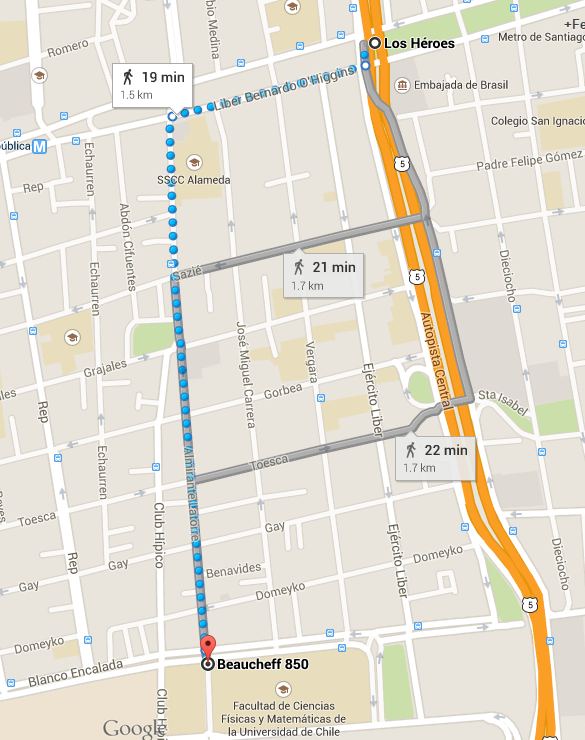
\includegraphics[width=200pt]{../images/google_map.png}}
\caption[Mapa de GoogleMaps]{Mapa que indica posibles rutas a seguir (caminando) desde beaucheff 850 a la estación de metro Los Heroes. (obtenida desde \textit{maps.google.cl})}
\label{fig:google_map}
\end{figure}

Lo anterior sugiere que las imágenes distorsionadas tienden a ser imprecisas y dependen de quien las observa. 

\end{description}	 

Otra manera de diferenciar la visualización es según el nivel de interacción que ésta presenta. Según esto tenemos

\begin{description}
	\item[Visualización estática] no permite interacción, muy parecido a una imagen.
	\item[Visualización dinámica] permite interacción, aquí el usuario puede consultar en la visualización y en consecuencia, interactuar con la aplicación de visualización en lugar de usar un menú, pudiendo llegar incluso a tener aplicaciones que son totalmente dirigidas a través de su visualización.
\end{description}

% sección 1.3 del libro | relación de visualización y otros campos
% sección 1.3.1 diferencia entre visualización y computación gráfica

%La visualización se relaciona mucho con la computación gráfica pero no son lo mismo. En un inicio, la visualización fue considerada un sub-campo dentro de la computación gráfica principalmente porque la visualización usa gráficos generados por computadoras mostrar información por medio de imágenes. Aquí las técnicas gráficas son usadas como medio de comunicación.

%Más allá de los gráficos utilizados, lo verdaderamente importante es el aspecto de toda visualización es su conexión con los datos. La computación gráfica se concentra principalmente en objetos gráficos y la organización de primitivas gráficas; la visualización va un paso más allá dado que son basadas en los datos subyacentes. Según todo lo anterior, se puede pensar en la visualización como la aplicación de gráficos para mostrar datos que se logra por medio de un mapeo a primitivas gráficas que luego de renderizar se obtiene la visualización.

%render: cálculo que se hace para generar una imagen.

La visualización enfatiza muchos aspectos de otras disciplinas, abarcando áreas como la computación gráfica, psicología perceptual, interacción humano-computador, base de datos, estadística, y minería de datos, entre otras. 
%La computación gráfica puede ser usada para definir y generar una vista para comunicar la información, la interacción humano-computador establece una base para el proceso de intercambio de datos entre el usuario y el software. Por último la sicología perceptual ayuda a generar visualizaciones efectivas. 
	
% visualización científica vs visualización de información.
% sección 1.3.2 del libro
Hoy en día existen dos corrientes de visualización, una científica y otra de información. Ambas proveen representaciones de datos, pero la diferencia más característica es que estos datos suelen ser a menudo diferentes. 

% sección 1.4 El proceso de visualización
\paragraph{El proceso de visualización} \hfill \\

Los datos utilizados para una visualización pueden ser simples o complejos en su estructura, y quien observa podría tener distintos objetivos sobre esos datos (buscar algo interesante como anomalías, tendencias, confirmar una hipótesis, mostrar resultados de análisis a una audiencia, etc). Por esto, uno de los primeros pasos para llevar a cabo una visualización es realizar un mapeo desde los datos a la vista (ver figura \ref{fig:proc_visualizacion}), y no hay una única forma de hacerlo. 

%La interfaz de usuario está compuesta de componentes que se asocian con la necesidad de ingresar, presentar, monitorear, analizar y computar datos. Pueden ser de muchas formas, incluso representaciones visuales de los datos para facilitar la selección requerida. Las visualizaciones pueden ofrecer mecanismos de traducción de datos para ofrecer vistas  y formatos más intuitivos para que los usuarios puedan llevar a cabo sus tareas. Lo anterior significa que los datos (o atributos de estos) son utilizados para definir objetos gráficos como puntos, líneas y formas; y sus atributos como tamaño, posición, orientación y color.

% Imagen de proceso de visualización
\begin{figure}[h] %[h] para here [b] para bottom [t] para top
\makebox[\textwidth]{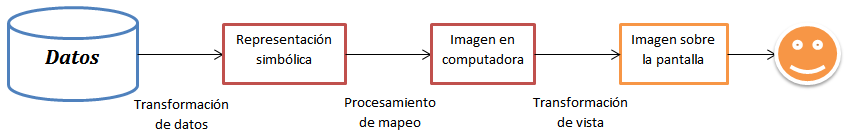
\includegraphics[width=300pt]{../images/proceso_visualizacion.png}}
\caption{Proceso de visualización. }
\label{fig:proc_visualizacion}
\end{figure}

En la figura \ref{fig:proc_visualizacion} se observa un proceso de visualización genérico que describe a grandes rasgos las etapas presentes. Según esto las etapas son:

\begin{description}
	\item[Transformación de datos] En esta etapa se realizan una o más operaciones\footnote{Todo lo relacionado con el pre-procesamiento de datos} (limpieza, correcciones, etc) que convierten los datos desde la fuente de datos en una representación simbólica en la computadora. 
	
	\item[Procesamiento de mapeo] Cada representación simbólica es asociada a un objeto gráfico cuyas características suelen representar atributos de cada elemento obtenido en el paso anterior. El conjunto de estos objetos producen una imagen en un computador.
	
	\item[Transformación de vista] Cada imagen puede ser transformada según requerimientos que tenga el usuario o si hay un grado de interación, éste tiene la posibilidad de hacerlo en el momento que lo requiera.
	
\end{description}

% capitulo 5 y 6 habla de mapeos de datos.
% capitulo 12. Estrategias para seleccionar mapeos eficientes.

%Otro componente importante dentro del proceso son los controles de interacción para las vistas y mapeos de variables (atributos o parámetros). Mientras que en un principio las visualizaciones fueron objetos estáticos, las visualizaciones modernas son procesos dinámicos donde el usuario controla virtualmente todas las etapas  del procedimiento, desde la selección y control a la definición de color y refinación de la vista. 
Es importante decir que no hay una fórmula que garantice la efectividad de una visualización. Diferentes usuarios, con diferentes formaciones, habilidades perceptuales y preferencias, tendrán difrentes opiniones sobre una visualización. La tarea que deban realizar los usuarios afectará también la utilidad de la visualización.

La visualización es a menudo una parte de un proceso más grande como análisis de datos, descubrimiento de conocimiento o análisis visual.

El proceso de comenzar con datos y generar una imagen es descrito como \textit{pipeline}, que se define como una secuencia de etapas que puede ser estudiada independientemente en términos de algoritmos, estructura de datos y sistema de coordenadas. %Esos procesos o pipeline son diferentes para computación gráfica, visualización y descubrimiento de conocimiento pero se parecen mucho. 

A continuación se muestra una descripción del pipeline de visualización. Las etapas son descritas en el mismo orden en que son ejecutadas durante el proceso (ver figura \ref{fig:pipeline_visualizacion}).
.

% sección 1.4.1 El canal de la computación gráfica

% sección 1.4.2 El canal de la visualización


% Imagen de pipeline de visualizacion
\begin{figure}[h] %[h] para here [b] para bottom [t] para top
\makebox[\textwidth]{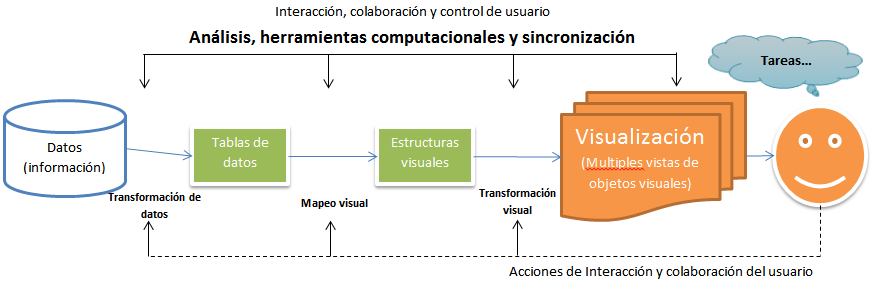
\includegraphics[width=350pt]{../images/pipeline_visualizacion.png}}
\caption[Pipeline de visualización]{Ejemplo de pipeline de visualización. Muestra la idea esencial de un pipeline, que es transformar los datos en una representación interna dentro del computador para luego usar un paradigma visual para desplegarlo sobre una pantalla.}
\label{fig:pipeline_visualizacion}
\end{figure}


\begin{description}
	\item[Modelado de datos] \hfil \\
Si están en un archivo o en una base de datos, tienen que estar  estructurados. Esta estructura se evalúa en base a dos conceptos, sintaxis, relacionada con el significado de su representación y semántica, visto como la relación existente entre registros. Además se realiza una limpieza de los datos, aquí se pueden utilizar varias estrategias (eliminar registros malos, valor sentinela, reeplzar por valor más cercano, etc) para luego identificar cada uno de los tipos de datos existentes (Ordinal,Nominal). Por último, si hay datos faltantes puede recurirse a la interpolación.

%El nombre, tipo, rango y semántica de cada atributo o campo de un dato tiene que estar disponible en un formato que asegure rápido acceso y fácil modificación.
	
	\item[Selección de datos] \hfill \\
Se relaciona con la identificación del subconjunto de datos que serán potencialmente visualizados. Esto puede ocurrir totalmente bajo el control del usuario o a través de un algoritmo automatizado.

	\item[De los datos a mapeo visual] \hfill \\
Este es lo más importante dentro del pipeline, la realización del mapeo de los valores de los datos a entidades gráficas con  sus respectivos atributos. Esta etapa usualmente involucra un procesamiento previo de los datos a ser mapeados como escalamiento, desplazamiento, filtrado, interpolación, entre otros. Esta etapa es muy dependiente de la librería subyacente en la visualización.

	\item[Configuración de parámetros de la escena] \hfill \\
Como en las gráficas tradicionales, el usuario tiene que especificar muchos atributos de la visualización que son relativamente independiente de los datos. Esto se refiere a configurar parámetros como los colores (para diferentes dominios, ciertos colores tienen significados claramente definidos), o especificación de luz si se tratase de una visualización 3D, etc.

	\item[Renderizado o generación de la visualización] \hfill \\
La proyección específica o el renderizado a ser utilizado para los objetos a visualizar depende del mapeo que se ha utilizado. En este aspecto, la mayoria de las visualizaciones solo requieren dibujar lineas y poligonos uniformemente pintados. Junto a mostrar los datos en si mismo, muchas también incluyen información suplementaria para facilitar la interpretación, como ejes, anotaciones, entre otros.

\end{description}

% sección 1.4.3 El proceso de descubrir conocimiento

% sección 1.4.4 El rol de la percepción

%\paragraph{El rol de la percepción}

%En todas las visualizaciones, un aspecto crítico relacionado al usuario son las habilidades y limitaciones de su sistema visual. Si el objetivo principal de la visualización es transmitir información por medio de imágenes es esencial considerar la percepción. Los usuarios interactuan con las visualizaciones según como ellos la ven y la interpretan. Entendiendo como vemos deberíamos ser capaces de construir mejores vistas, o al menos evitar producir las que no aportan valor. Algunas de las cosas relevantes que se deben tener en cuenta son: el 8\% de los hombres tiene algún problema con los colores, lo que quiere decir que una herramienta de visualización debería permitir cambiar los colores de los objetos que aparecen en la pantalla. Además los colores dependerán de la deficiencia del usuario y de la visualización que se está tratando transmitir.

% ver capitulo 3: Percepción

%El sistema perceptual recibe datos y los procesa de varias formas. El primer proceso es \textit{procesamiento pre-atencional}, un rápido sistema de alto rendimiento que rápidamente identifica diferencias en, por ejemplo, colores y texturas. Además de este hay otras características que el sistema perceptual debe manejar, como la orientación de una línea, largo, ancho, tamaño de un objeto, curvatura, agrupamiento, y movimiento.

%Al entender la percepción visual tenemos ciertas pautas. Por ejemplo, en 1912 la \textit{Gestalt School of Psychology} comenzó a intentar definir un conjunto de leyes según las cuáles percibimos patrones. Estas leyes incluyen reglas de proximidad, similaridad, continuidad, simetría, primer plano, fondo, y tamaño.

% sección 1.5 Convenciones de código
% sección 1.6 el diagrama de dispersión
% sección 1.7 el rol del usuario

\paragraph{El rol del usuario} \hfill \\

El usuario puede estar envuelto en la mayoría de las etapas del pipeline de visualización. Un aspecto importante desde este punto de vista es la intensión del usuario, según esto, es útil categorizar la visualización basados en los propósitos que ésta tendrá. Según esto surgen las siguientes categorías:

\begin{description}
	\item[Exploración] \hfill \\
El usuario posee un conjunto de datos y quiere examinarlos para averiguar su contenido y/o si una característica particular (o conjunto de estas) está presente o ausente.

	\item[Confirmación] \hfill \\
El usuario ha determinado o planteado una hipótesis relacionada con una característica de los datos y quiere usar la visualización para verificarla.

	\item[Presentación] \hfill \\
El usuario está intentando transmitir algún concepto o conjunto de hechos a una audiencia.
\end{description}


	%\paragraph{Origenes de datos}
	%Capitulo 2	
	%\paragraph{Percepción}
	%Capitulo 3
	%\paragraph{Interacción}
	%Capitulo 10 y 11
    
	%\paragraph{Técnicas para datos geoespaciales}
    
    \newpage
    \subsection{Análisis de datos}\label{sec:Analisis_datos}

	A continuación se detalla la forma en que funciona el sistema de transporte público que origina los datos, como se estima el proceso de bajada y por último los detalles de las tablas obtenidas posterior a la estimación. Tanto la metodología como los supuestos aquí explicados son expuestos y propuestos por Munizaga y Palma (2012) \cite{Procesamiento_datos}.
	
	\subsubsection{Sistema tarifario}
En Santiago de Chile, el sistema AFC utilizado corresponde a las tarjetas de pago, donde en buses es el único método disponible y en metro es el más utilizado.

El sistema de pago en Transantiago es tal que cada pasajero paga una tarifa cuando accede al sistema, que permite a él o ella hacer tres transbordos dentro de las dos horas siguientes al pago. La estructura de pago es diferente entre el metro y buses. En buses, el único sistema de pago es mediante la tarjeta de pago (llamada comercialmente tarjeta bip!), mientras que en metro, es posible comprar un ticket o usar la tarjeta bip!, sin embargo el porcentaje de usuarios que compra el ticket es de aproximadamente 3\%.
%Por otro lado el pago en metro difiere, ligeramente más alto, para los horarios de alta demanda, entonces si un pasajero usa primero bus y luego transborda a metro, la diferencia entre ambas líneas de transporte es cobrada cuando la persona accede a éste último.

% actualizar datos

El sistema se caracteriza por tener cerca de 300 rutas de buses, 6000 buses disponibles agrupados en 6 operadores\footnote{Un operador es una empresa que se encarga de prestar servicio a una zona de santiago.}, aproximadamente 10.000 paraderos y una cifra que bordea los 150 kilómetros de rieles para el metro. 

Dada la alta demanda que ha experimentado, se crearon 150 zonas físicas llamadas ``zona paga" que están equipadas con sistema de pago (validadores) de vehículo donde el pasajero paga cuando entra a la estación, lo cual incrementa la eficiencia de las subidas a los buses pero genera una dificultad para determinar cual bus de todos los que allí se detienen tomó un usuario. Es importante decir que estas estaciones de buses operan durante los horarios de alta demanda en puntos de congestión identificados previamente.

Todas las transacciones bip! Son guardadas en una base de datos que contiene información sobre los operadores y el instante en que la transacción fue hecha. Lo anterior se lleva a cabo por cada pasajero acercando su tarjeta al validador cuando ingresa al bus, zona paga o metro. Cada validador adjunta a cada transacción que realiza un id asociado a el y que está a su vez, asociado con un bus, zona paga o metro. La información recolectada por cada transacción incluye: \textbf{id de la tarjeta}, \textbf{tipo}\footnote{puede ser comercial o estudiante.},  \textbf{código de bus o sitio donde se realizó la transacción}, \textbf{fecha y hora}, \textbf{monto de pago}. La posición espacial de la transacción puede ser conocida directamente para las zonas paga y las estaciones de metro dado que son conocidas con anterioridad, para las transacciones hechas en buses es posible pero no está disponible en la base de datos de transacciones.

%Todas las semanas se realizan alrededor de 35 millones de transacciones con cerca de 3 millones de tarjetas bip!. Por otro lado, 

Otra base de datos contiene información sobre la localización de todos los buses, como la \textbf{latitud}, \textbf{longitud}, \textbf{tiempo}, \textbf{fecha} y \textbf{velocidad instantánea}. Estos datos son obtenidos a intervalos de 30 segundos y son asociados a cada bus a través de un número de placa y código de operador.

Cruzando la información de transacción y posición de las bases de datos por cada placa de bus o código de metro/zona paga y tiempo, es posible identificar la localización espacial donde la transacción es realizada. Es así como en datos analizados del año 2009 y 2010 se logra una estimación en el 98,5\% y 99,9\% de los casos respectivamente.\cite{Procesamiento_datos}.

\subsubsection{Estimación de bajadas}

Como en el sistema de tarifa solo se validan las subidas, es necesario estimar los puntos de bajadas de las transacciones. Es aquí donde Munizaga y Palma (2012)\cite{Procesamiento_datos} utilizan una serie de supuestos para entender el comportamiento general de los usuarios dentro del sistema. Para lo anterior utilizan la definición de viaje dada por \textit{Ortúzar y Willumsen, 2011}\cite{Viaje}:

\begin{center}
	\textit{``Un viaje se define como un movimiento desde un punto de origen a un punto de destino donde se realiza una actividad"}
\end{center} 

Esta definición origina la consideración de etapas dentro de un viaje, una etapa es la utilización de un servicio en particular (bus o metro), entonces la combinación de estos hecha hasta que el usuario llegue al lugar donde debe llevar a cabo su actividad es lo que entendemos como un viaje. Es importante notar que no se consideran los cambios entre líneas de metro.

Básicamente la idea es seguir una cadena de viajes de una tarjeta e identificar la posición de bajada (de bus o metro) mirando la posición y el tiempo de la próxima subida de esta tarjeta. Esto es solamente posible cuando la actual y siguiente transacción tiene información de posición, la cual es tomada de la base de datos de localización automática de vehículos. En el caso de la última transacción del día, se asume que el destino es cercano al punto donde el primer viaje del día comienza, encontrando así un viaje cíclico diario para los usuarios particulares. Si hay solo un viaje por tarjeta, no es posible inferir con solo un día de información.

Los supuestos para llevar a cabo esta estimación son: 
\begin{itemize}
	\item Después de un viaje, el origen del siguiente determina el destino del primero. \cite{Supuesto_Barry}
	\item al final del día, los usuarios van a volver a la estación donde abordaron en el primer viaje del mismo día. \cite{Supuesto_Barry}
	\item Cada tarjeta corresponde a un usuario. \cite{Procesamiento_datos}
	\item Se asume que una persona camina hasta la siguiente parada un máximo de 1.000 metros \cite{Procesamiento_datos}
	\item Si el tiempo de transbordo\footnote{entendido como el tiempo entre que se bajó de un servicio y se subió al siguiente.} es inferior a 30 minutos, entonces este último servicio forma parte del mismo viaje, de lo contrario se considera como uno nuevo.\cite{Procesamiento_datos}
\end{itemize}

Según todo lo anterior Munizaga y Palma (2012)\cite{Procesamiento_datos} son capaces de estimar cerca del 80\% de los datos utilizados. Dado que es necesario conocer esta información, se restringe los datos al porcentaje de datos que forman parte del resultado exitoso.

%\subsubsection{Identificación de actividades}
% evaluar si esto es necesario ya que pareciera que no.
% hablar de paper de deteccion de actividades.

\subsubsection{Descripción de los datos}

El procedimiento anterior ya se encuentra realizado para los datos comprendidos entre el 14 de abril de 2013 al 20 de abril de 2013 por lo que será este tramo el que será utilizado para realizar el análisis espacial y dado que es requerido conocer cada etapa que realiza una persona, se opta por utilizar la tabla de etapas en donde una fila representa una etapa de un viaje determinado. Esta tabla actualmente contiene 42 columnas producto de diversos análisis que se han realizado con ellas pero que no son todos útiles para el desarrollo de esta memoria por lo que se omite la mayoría. En la tabla \ref{tabla:etapa} se listan los campos a ser utilizados para el procesamiento de los datos.

\begin{table}[h]
\begin{center}
  \begin{tabular}{| l | p{7cm} |}
    \hline
    Nombre campo & Descripción \\ \hline \hline
%    tiempo\_subida & fecha y hora en que se realizó una validación en el sistema  \\ \hline
    id & identificador de la tarjeta que realizó la validación \\ \hline
%    pago &  \\ \hline
%    x\_subida &  \\ \hline
%    y\_subida &  \\ \hline
%    tipo\_transporte &  \\ \hline
%    serviciosentidovariante &  \\ \hline
%    tipo\_dia &  \\ \hline
    nviaje &  Indica el número de viaje asociado al id de la tarteja de pago\\ \hline
    netapa &  lugar que ocupa la etapa dentro de un viaje.\\ \hline
%    x\_bajada &  \\ \hline
%    y\_bajada &  \\ \hline
%    tiempo\_bajada &  \\ \hline
    par\_subida & Indica el paradero en donde abordo el servicio. \\ \hline
    par\_bajada & Señala el paradero de donde descendió del servicio. \\ \hline
%    comuna\_subida &  \\ \hline
%    comuna\_bajada &  \\ \hline
%    zona\_subida &  \\ \hline
%    zona\_bajada &  \\ \hline
%    distonroutesubidabajada &  \\ \hline
%    disteuclidsubidabajada &  \\ \hline
%    distonrouteparsubidaparbajada &  \\ \hline
%    disteuclidparsubidaparbajada &  \\ \hline
%    serv\_un\_zp2 &  \\ \hline
%    sitio2 &  \\ \hline
%    tiempo2 &  \\ \hline
%    media\_hora &  \\ \hline
%    tiempo\_trasbordo &  \\ \hline
%    dist\_trasbordo &  \\ \hline
%    tiempo\_caminata &  \\ \hline
%    tiempo\_espera &  \\ \hline
%    tiempo\_etapa &  \\ \hline
%    tiempo\_espera\_estimado &  \\ \hline
%    escolar &  \\ \hline
%    factor\_exp\_etapa &  \\ \hline
%    nbusesanteriores &  \\ \hline
%    tiempo\_busanterior &  \\ \hline
%    busanterior1er &  \\ \hline
%    busanterior2do &  \\ \hline
%    busanterior3er &  \\ \hline
%    tipocorte &  \\ \hline
%    proposito &  \\ \hline
  \end{tabular}
\end{center}
\caption{Atributos a utilizar de la tabla ETAPAS}:
\label{tabla:etapa}
\end{table}

No se descarta que una vez realizada la etapa de visualización puedan requerirse más datos con respecto a cada etapa, como puede ser la fecha y hora, tipo de transporte, entre otros.

Además de la tabla de etapas es necesario conocer todos los paraderos disponibles con el fin de poder realizar la interpolación, por lo que también se utiliza la tabla REDPARADAS (ver tabla \ref{tabla:paradero}) en conjunto con la tabla ESTACIONES\_METRO (ver tabla \ref{tabla:estacion_metro}) que contiene los datos de las estaciones de metro, éstos serán tratados de manera indistinta ya que tanto los paraderos de bus como las estaciones de metro funcionan como puntos de origen o destino en una etapa.

La tabla REDPARADAS contiene 23 columnas con una serie de datos asociados a cada paradero existente en sistema público de transporte de Santiago de Chile. Muchas de éstas han sido agregadas para diversos análisis previos que no se relacionan con esta memoria. Para efectos de este trabajo esta tabla presenta 3 atributos importantes a destacar descritos en la tabla \ref{tabla:paradero}. 

La tabla ESTACION\_METRO contiene 20 atributos, y al igual que la tabla REDPARADAS, la mayoría de sus campos fueron agregados para la ejecución de análisis previos. Los atributos relevantes son descritos en la tabla \ref{tabla:estacion_metro}.

\begin{table}[h]
\begin{center}
  \begin{tabular}{| l | p{7cm} |}
    \hline
    Nombre campo & Descripción \\ \hline \hline
    codigousuario & identificador único de paradero, ej:PJ156 \\ \hline
    x & posición en eje horizontal dentro del sistema de coordenadas cartesiana utilizado para la georeferenciación \\ \hline
    y & posición en eje vertical dentro del sistema de coordenadas cartesiana utilizado para la georeferenciación \\ \hline
  \end{tabular}
\end{center}
\caption{Atributos a utilizar de la tabla REDPARADAS}:
\label{tabla:paradero}
\end{table}

\begin{table}[h]
\begin{center}
  \begin{tabular}{| l | p{7cm} |}
    \hline
    Nombre campo & Descripción \\ \hline \hline
    codigosinlinea & Nombre de la estación de metro \\ \hline
    x & posición en eje horizontal dentro del sistema de coordenadas cartesiana utilizado para la georeferenciación \\ \hline
    y & posición en eje vertical dentro del sistema de coordenadas cartesiana utilizado para la georeferenciación \\ \hline
  \end{tabular}
\end{center}
\caption{Atributos a utilizar de la tabla ESTACION\_METRO}:
\label{tabla:estacion_metro}
\end{table}

    \subsection{Conclusiones}
    
	Es importante destacar que la particularidad del estudio radica en que el grafo formado para construir las estructuras espaciales no representa viajes sino actividades urbanas que realizan las personas, construyendo así una red social formada por actividades urbanas.
	
	Tanto las definiciones de propiedades globales como las formulas definidas aquí serán ocupadas tal cual aparecen de manera de más adelante poder comparar los resultados obtenidos con los mostrados en el artículo, que está basado en el sistema de transporte público de Singapur.

	El \textit{factor de amortiguación} será ajustado al propuesto por Chen Zhong et al. (2014)\cite{Estructura_urbana}, no es campo de esta memoria el considerar variaciones de este factor, por lo tanto será fijado en $0.85$.

	Se utilizará el framework \textit{map equation}	 para llevar a cabo la generación de comunidades dado que plantea el mejor desempeño según Lancichinetti y Fortunato (2009) \cite{Comparar_generador_comunidad}.
	
La variante de interpolación escogida, al igual que en Chen Zhong et.al (2014) corresponde a la \textit{Inverse Distance Weighting}(\textit{IDW}) con un $\lambda=2$ dado que no se hacen supuestos adicionales a los propuestos.
	
%\todo{explicar que se usará georeferenciación, que estándar, etc..}	
	
    Este trabajo al igual que el artículo en el que está basado, utiliza los datos generados a partir del uso de tarjetas inteligentes del transporte público, con la salvedad de que aquí corresponden al sistema de transporte de Santiago de Chile, con estos se construirá  la red espacial para la posterior construcción de las estructuras descritas (centros, centros de flujo y bordes).
	
	Como los datos de Santiago de Chile presentan las mismas características luego de aplicar el método de estimación de Munizaga y Palma (2012), se observa que estos son aptos para replicar el análisis hecho en Singapur. Es importante decir que este procesamiento fue realizado con anterioridad a este trabajo y aquí se documenta con fines explicativos.

La efectividad de la visualización depende de las preferencias  y nivel de entrenamiento de los usuarios por lo que se debe considerar la elaboración del perfil de los usuarios que usarán la aplicación. 

Al momento de diseñar la visualización no es necesario considerar la distorsión producida en las imagenes bidimensionales presentes en un mapa producto de la proyección existente (3D a 2D) dado que el nivel de detalle que se requiere en las vistas se relaciona a nivel de ciudad, no de calle. 

La estrategia para el proceso de visualización queda establecida en la sección \ref{sec:contr_y_rep_red} ``Construcción y representación de la red'', por lo que no es necesario definir una.

	Para la realización de las vistas se debe tener presente la percepción de los usuarios, la intención de ésto y como estos aspectos afecta cada visualización.
	
	En estos momentos existen dos vistas candidatas a ser desplegadas en la versión final. Estas son:
	
	\begin{itemize}
		\item Visualización del mapa de la ciudad de Santiago de Chile  donde se muestra una partición de ésta por el procedimiento que genera las comunidades.
		\item Visualización del mapa de la ciudad de Santiago de Chile  que indica aquellas áreas que son consideradas centros y centros de flujo.
	\end{itemize}		
	
	A partir de todo lo expuesto, el aporte de este trabajo a lo ya existente se resume en:
	
	\begin{itemize}
	\item Validación del modelo propuesto por Cheng Zhong et al. (2014) \cite{Estructura_urbana} por medio de la aplicación de su metodología a otra fuente de datos real (sistema de transporte público de Santiago de Chile).
	\item Diseño de una herramienta de visualización que permite observar los resultados obtenidos por la metodología de Cheng Zhong et al.
	\item Contribuir al análisis de la información provista por los datos pasivos del transporte público de Santiago de Chile con una herramienta que permite observar una perspectiva diferente a lo realizado previamente.
	
	\end{itemize}
	
    \newpage
    %================================================================================================================
    \section{Estrategia de procesamiento}

%    Como se explicó al final del capitulo 4, esta sección es abordada parcialmente dado que la investigación que se lleva a cabo es extensa. Se nombra lo realizado y al final se listan las tareas pendientes que serán desarrolladas durante el período previo al inico del siguiente semestre (2015-1) con el fin de tener holgura frente a posible eventualidades.
    
	En esta sección se describen las acciones llevadas a cabo para obtener los archivos necesarios para ser analizados y visualizados, es decir, para elaborar el grafo y calcular los indicadores descritos en la sección \ref{sec:Analisis_bibliografia}. Para lo anterior primero se detallan las herramientas que se utilizarán y luego se explican las acciones llevadas a cabo.

	\subsection{Herramientas a utilizar}
	
	Todos los procesamientos son llevados a cabo en un Notebook con sistema operativo Debian GNU/Linux 7.8 con 3GB de memoria RAM, 40 GB de espacion en disco duro de 5400RPM y un procesador Intel Core i5 4200M de 2.5 GHz.
	La base de datos que contiene las etapas, paraderos y estaciones de metro se encuentra en un Sistema Gestor de Base de Datos (\textit{SGBD}) \textbf{Postgres} versión 9.1 y para gestionar los datos se posee una interfaz gráfica (\textit{GUI}) llamada \textit{PgAdmin III} cuya versión es 1.18.1 con la cuál se manipulan los distintos requerimientos al SGBD. 
	La construcción de comunidades será realizada mediante la herramienta \textit{mapEquation}\footnote{http://www.mapequation.org}.
	
	Por último, se usa el paquete \textit{igraph}\footnote{http://igraph.sourceforge.net/} como libreria del lenguaje C para calcular los indicadores $C_{intermediacion}$ y $PageRank$, además de las propiedades globales del grafo.
	 
	Aquellas funcionalidades adionales que se requieran serán hechas con alguna de las herraminentas aquí nombradas o mediante scripts hechos en el lenguaje de programación C o PHP.
	
	La siguiente sección (y en adelante) da por hecho la existencia de una base de datos de nombre 'memoria' que contiene las siguientes tablas:

	\begin{itemize}
		\item etapas:	 Registros de un tramo realizado
		\item viajes:	 Registros de viajes (conjunto de etapas).
		\item red\_paradas:	 Registros de paraderos.
		\item etapas\_utiles: Registros de la tabla etapa que aprueban el filtrado de datos.
		\item viajes\_utiles: Registros de la tabla viaje que aprueban el filtrado de datos.
		\item pajek\_por\_hora: Registros utilizados para generar los archivos pajek.
	\end{itemize}
	
	Para ver la estructura en detalle de cada tabla revisar anexo \ref{anexo:bd}.
	
	\subsection{Filtrado de datos}
	
	En este paso se quitan aquellos datos que no cumplen con el requisito de tener un paradero de bajada (o subida) asociado, para esto se extraen los datos que cumplen con la siguiente consulta en lenguaje \textit{SQL} (\textit{Structure Query Language}) y se guardan en la tabla con datos ya filtrados.
	
\begin{figure}[h]
\begin{center}
\begin{lstlisting}[breaklines=true, language=SQL]
	INSERT INTO etapa_util
	SELECT id, nviaje, netapa, par_subida, par_bajada 
	FROM etapas 
	WHERE par_subida IS NOT NULL OR par_bajada IS NOT NULL;
\end{lstlisting}
\end{center}
\caption{Consulta para quitar etapas sin paradero de bajada.}
\label{fig:limpiar_datos_etapa}
\end{figure}
	
	Los resultados de la consulta anterior (figura \ref{fig:limpiar_datos_etapa}) son almacenados en la tabla etapa\_util que contiene solo los campos a ser utilizados.
	
	Se realiza el mismo procedimiento para la tabla de viajes como se puede observar a continuación (figura \ref{fig:limpiar_datos_viajes}) pero guardandose en una tabla distinta llamada viaje\_util.

\begin{figure}[h]
\begin{center}
\begin{lstlisting}[breaklines=true, language=SQL]
	INSERT INTO viaje_util
	SELECT codigousuario, x, y  
	FROM redparadas
	WHERE x IS NOT NULL AND y IS NOT NULL;
\end{lstlisting}
\end{center}
\caption{Consulta para quitar atributos innecesarios de la tabla REDPARADAS.}
\label{fig:limpiar_datos_viajes}
\end{figure}	


\begin{figure}[h]
\begin{center}
\begin{lstlisting}[breaklines=true, language=SQL]
	SELECT codigousuario, x, y  
	FROM redparadas
	WHERE x IS NOT NULL AND y IS NOT NULL;
\end{lstlisting}
\end{center}
\caption{Consulta para quitar atributos innecesarios de la tabla REDPARADAS.}
\label{fig:limpiar_datos_redparadas}
\end{figure}	
	
\begin{figure}[H]
\begin{center}
\begin{lstlisting}[breaklines=true, language=SQL]
	SELECT codigosinlinea, x, y  
	FROM estacion_metro
	WHERE x IS NOT NULL AND y IS NOT NULL;
\end{lstlisting}
\end{center}
\caption{Consulta para quitar atributos innecesarios de la tabla ESTACION\_METRO.}
\label{fig:limpiar_datos_estacion_metro}
\end{figure}	

Al finalizar esta etapa se obtienen 3 tablas con los datos necesarios para llevar a cabo el cálculo de las siguientes instrucciones.

	\subsection{Construcción de la red}
	
Con los datos de la tabla ETAPA se construye una matriz origen destino donde cada celda $C_{ij}$ denota el volumen de etapas realizadas desde el área asociada al paradero $i$ al área asociada al paradero $j$. Lo anterior se realizará utilizando la herramienta $R$ con el paquete \textit{i-graph}.

%\begin{figure}[h]
%\begin{center}
%\begin{lstlisting}[breaklines=true, language=R]
%	asd
%\end{lstlisting}
%\end{center}
%\caption{Código para construir matriz Origen-Destino}
%\label{fig:matriz_o_d}
%\end{figure}	

    \subsection{Trabajo pendiente}
    
    A continuacion se listan las tareas pendientes de esta sección:
    
    \begin{itemize}
    	\item	Cálculo de centralidades.
    		\begin{itemize}
    			\item Centralidad de intermediación
    			\item PageRank
    		\end{itemize}
    	\item Cálculo de bordes y generación de comunidades
    	\item Realización de interpolación espacial
    	\item Corrección de bordes
    \end{itemize}
    
    Como se dijo anteriormente, serán realizadas durante el período previo al inicio del semestre 2015-1.
    
	\subsection{Solo punteos}    
    
    Antes de hacer cualquier cosa con los datos debemos eliminar aquellos que no tienen paradero de subida ni de bajada.
    
\begin{lstlisting}[breaklines=true, 
				   language=SQL, 
				   caption=Generación de arcos,
				   label=fig:generacion_arcos]	
DELETE FROM etapas WHERE par_subida IS NULL OR par_bajada IS NULL;
\end{lstlisting}
    La eliminación demoró 879228.976 ms (14.65 m) y sequitaron 6.963.870 registros sin paradero de bajada y 5434 que no tienen paradero de subida.    
    
consulta para obtener los arcos con pesos 
	
\begin{lstlisting}[breaklines=true, 
				   language=SQL, 
				   caption=Generación de arcos,
				   label=fig:generacion_arcos]		
su postgres

psql memoria
	
-- lo guardamos como un CSV
copy (SELECT par_subida, par_bajada, COUNT(*) AS peso 
	  FROM etapas AS prueba 
	  GROUP BY par_subida, par_bajada) 
To '/var/tmp/dia.csv' with CSV;


-- V2 lo guardamos como un CSV. No funciona parece que hay codigos que no estan en la tabla de paraderos. Esta consulta no se ocupo (con acento en la o)
copy (SELECT subida.nombre, bajada.nombre, arcos.peso
	 FROM (SELECT par_subida, par_bajada, COUNT(*) AS peso 
	  	   FROM etapas AS prueba 
	  	   GROUP BY par_subida, par_bajada) AS arcos
	  	   LEFT JOIN redparadas AS subida ON arcos.par_subida = subida.codigo 
	  	   LEFT JOIN redparadas AS bajada ON arcos.par_subida = bajada.codigo) 
To '/var/tmp/dia.csv' with CSV;
\end{lstlisting}

	La ejecución de esta consulta demoró 2187691.139 ms (36.46 m) y se generaron 644.761 filas, lo que indica la cantidad de arcos presentes. Esto es sobre todos los viajes existentes.
	
	Ahora se genera el mismo archivo pero con un rango horario de mañana (05:00-12:00) y otro rango horario de tarde  (16:00-21:00). Para lo anterior se generan dos indices para mejorar el rendimiento de la consulta.
   
    Antes de consultar se crea un índice sobre el campo tiempo\_subida para mejorar el rendimiento.

\begin{lstlisting}[breaklines=true, 
				   language=SQL, 
				   caption=Creación de índice,
				   label=fig:generacion_indice]	
CREATE INDEX hora_subida ON etapas (extract(hour from tiempo_subida));
\end{lstlisting}

Su creación demoró 294591.532 ms (4.91 min)

Luego se genera el archivo con datos de la mañana y tarde según los períodos definidos mas arriba.

\begin{lstlisting}[breaklines=true, 
				   language=SQL, 
				   caption=Generación de arcos horario mañana,
				   label=fig:generacion_arcos_manana]		
su postgres

psql memoria
	
// lo guardamos como un CSV
copy (SELECT par_subida, par_bajada, COUNT(*) AS peso 
	  FROM etapas AS prueba 
	  WHERE extract(hour from tiempo_subida) BETWEEN 05 AND 12 
	  GROUP BY par_subida, par_bajada) 
To '/var/tmp/manana.csv' with CSV;
\end{lstlisting}

demoró 1221570.569 ms (20.34 min) y generó 457.015 arcos.

\begin{lstlisting}[breaklines=true, 
				   language=SQL, 
				   caption=Generación de arcos horario tarde,
				   label=fig:generacion_arcos_tarde]		
su postgres

psql memoria
	
// lo guardamos como un CSV
copy (SELECT par_subida, par_bajada, COUNT(*) AS peso 
	  FROM etapas AS prueba 
	  WHERE extract(hour from tiempo_subida) BETWEEN 16 AND 21 
	  GROUP BY par_subida, par_bajada) 
To '/var/tmp/tarde.csv' with CSV;
\end{lstlisting}

demoró 953715.972 ms (15.9 min) y generó 438.672 arcos.

    Formato de archivo
    
	Ahora debemos crear el archivo de nodos, para ellos ocuparemos el formato PAJEK y uno script (crear\_archivo\_pajek.php) en php convierten el CSV creado en un archivo con ese formato.
	
	Investigar-----    
    
    Ahora debemos intercambiar los nombres por números. Para lo anterior ocuparemos la tabla redparadas. Vamos a correr el script "cambiar\_nombre\_pajek.php".
    
        
    correr infomap (por el momento estamos ocupando la app web)
    
    ./infomap --input-format='' -d -2
    
    opciones
    -i<s>, --input-format=<s> : Specify input format ('pajek', 'link-list', '3gram' or 'multiplex') to override format possibly implied by file extension.
    --map : Print the top two-level modular network in the .map format.
    --clu : Print the top cluster indices for each node.
    -2, --two-level : Optimize a two-level partition of the network.
    -d, --directed : Assume directed links.
    
    el calculo de lo indicadores se hace con el programa Gephi. 
    
    Explicar como conseguirlos y exportar los datos en un csv.
    
%	\subsection{Cálculo de centralidades}
	
%		\subsubsection{Centralidad de intermediación}
		
%		\subsubsection{PageRank}
	
%	\subsection{Cálculo de Bordes y Generación de comunidades}
%	La detección de los bordes será realizada usando la herramienta \textit{MapEquation}\footnote{www.mapequation.org}
%	\subsection{Interpolación espacial}
	
%	\subsection{Corrección de bordes}  
	
%	Para la corrección de bordes se utilizará el algoritmo $PageRank$
    
    %\newpage
    %================================================================================================================
    %\section{Trabajo realizado}
    
    %Aquí debo poner los análisis que he hecho sobre los datos.
    
    %\newpage
    %================================================================================================================
    %\section{Implementación}
    
    %\subsubsection{Visualiazación}

    %\newpage
    %================================================================================================================
    %\section{Conclusiones y trabajo futuro}
    
    
    \newpage
    %================================================================================================================
    \section{Bibliografía}

    \renewcommand{\section}[2]{} % Elimina el titulo "references"

    \bibliographystyle{plain}
    \bibliography{references}
    
    \newpage
    %================================================================================================================
	\section{Anexos}
	
		\subsubsection{Instalación de Postgres}
		
	Para instalar postgres en Debian GNU/Linux se deben ejecutar la siguiente secuencia de operaciones en la consola de comandos.
	
\begin{lstlisting}[breaklines=true, 
				   language=SQL,  
				   title=asd, 
				   caption=Instalacion de postgres,
				   label=fig:instalar_postgres]
# El usuario con el que se ejecuta este codigo 
# debe ser root.

# Instala el sistema gestor de base de datos Postgres, 
# un programa para interactuar con las bases de datos 
# (psql) y crea un usuario en el sistema de nombre 
# postgres.
apt-get install postgresql postgresql-client	

\end{lstlisting}

		\subsubsection{Creación de base de datos}\label{anexo:bd}
		
	El código mostrado a continuación crea la estructura de la base de datos requerida para este trabajo.
	
\begin{lstlisting}[breaklines=true, 
				   language=SQL,  
				   title=asd, 
				   caption=Instalacion de postgres,
				   label=fig:instalar_postgres]
# Se inicia sesion con el usuario postgres 
su postgres
# Se accede al programa para interactuar con la base de datos.
psql

# Se crea usuario y base de datos
CREATE USER felipe WITH PASSWORD 'felipe';
CREATE DATABASE memoria OWNER felipe;

# Se cierra psql
\q

# Se ingresa a la base de datos 'memoria'
psql memoria

-- crear tabla etapas
CREATE TABLE etapas (
    tiempo_subida timestamp without time zone,
    id bigint,
    pago smallint,
    x_subida double precision,
    y_subida double precision,
    tipo_transporte character varying(20),
    serviciosentidovariante character varying(500),
    tipo_dia character varying(10),
    nviaje integer,
    netapa integer,
    x_bajada double precision,
    y_bajada double precision,
    tiempo_bajada timestamp without time zone,
    par_subida character varying(30),
    par_bajada character varying(30),
    comuna_subida character varying(20),
    comuna_bajada character varying(20),
    zona_subida character varying(10),
    zona_bajada character varying(10),
    distonroutesubidabajada integer,
    disteuclidsubidabajada integer,
    distonrouteparsubidaparbajada integer,
    disteuclidparsubidaparbajada integer,
    serv_un_zp2 character varying(500),
    sitio2 character varying(50),
    tiempo2 timestamp without time zone,
    media_hora time without time zone,
    tiempo_trasbordo double precision,
    dist_trasbordo double precision,
    tiempo_caminata double precision,
    tiempo_espera double precision,
    tiempo_etapa double precision,
    tiempo_espera_estimado double precision,
    adulto integer,
    factor_exp_etapa double precision,
    nbusesanteriores integer,
    tiempo_busanterior timestamp without time zone,
    busanterior1er integer,
    busanterior2do integer,
    busanterior3er integer,
    tipocorte character varying(100),
    proposito character varying(100)
);

ALTER TABLE public.etapas OWNER TO felipe;

-- crear tabla de viajes
CREATE TABLE viajes (
    id character varying(20),
    nviaje integer,
    netapa integer,
    etapas character varying(1000),
    netapassinbajada integer,
    ultimaetapaconbajada integer,
    tviaje_seg double precision,
    tviaje_min double precision,
    dviajeeuclidiana_mts double precision,
    dviajeenruta_mts double precision,
    paraderosubida character varying(50),
    paraderobajada character varying(50),
    comunasubida character varying(20),
    comunabajada character varying(20),
    diseno777subida character varying(20),
    diseno777bajada character varying(20),
    tiemposubida timestamp without time zone,
    tiempobajada timestamp without time zone,
    periodosubida character varying(100),
    periodobajada character varying(100),
    tipodia character varying(10),
    mediahora time without time zone,
    contrato character varying(50),
    factorexpansion double precision,
    tiempomediodeviaje timestamp without time zone,
    periodomediodeviaje character varying(200),
    mediahoramediodeviaje time without time zone,
    tipodiamediodeviaje character varying(10),
    t_1era_etapa double precision,
    d_1era_etapa double precision,
    tespera_1era_etapa double precision,
    ttrasbordo_1era_etapa double precision,
    tcaminata_1era_etapa double precision,
    t_2da_etapa double precision,
    d_2da_etapa double precision,
    tespera_2da_etapa double precision,
    ttrasbordo_2da_etapa double precision,
    tcaminata_2da_etapa double precision,
    t_3era_etapa double precision,
    d_3era_etapa double precision,
    tespera_3era_etapa double precision,
    ttrasbordo_3era_etapa double precision,
    tcaminata_3era_etapa double precision,
    t_4ta_etapa double precision,
    d_4ta_etapa double precision,
    tespera_4ta_etapa double precision,
    ttrasbordo_4ta_etapa double precision,
    tcaminata_4ta_etapa double precision,
    op_1era_etapa character varying(10),
    op_2da_etapa character varying(10),
    op_3era_etapa character varying(10),
    op_4ta_etapa character varying(10),
    tipoop_1era_etapa character varying(15),
    tipoop_2da_etapa character varying(15),
    tipoop_3era_etapa character varying(15),
    tipoop_4ta_etapa character varying(15),
    serv_1era_etapa character varying(500),
    serv_2da_etapa character varying(500),
    serv_3era_etapa character varying(500),
    serv_4ta_etapa character varying(500),
    linea_metro_subida_1 character varying(100),
    linea_metro_subida_2 character varying(100),
    linea_metro_subida_3 character varying(100),
    linea_metro_subida_4 character varying(100),
    linea_metro_bajada_1 character varying(100),
    linea_metro_bajada_2 character varying(100),
    linea_metro_bajada_3 character varying(100),
    linea_metro_bajada_4 character varying(100),
    paraderosubida_1era character varying(50),
    paraderosubida_2da character varying(50),
    paraderosubida_3era character varying(50),
    paraderosubida_4ta character varying(50),
    tiemposubida_1era timestamp without time zone,
    tiemposubida_2da timestamp without time zone,
    tiemposubida_3era timestamp without time zone,
    tiemposubida_4ta timestamp without time zone,
    zona777subida_1era character varying(50),
    zona777subida_2da character varying(50),
    zona777subida_3era character varying(50),
    zona777subida_4ta character varying(50),
    paraderobajada_1era character varying(50),
    paraderobajada_2da character varying(50),
    paraderobajada_3era character varying(50),
    paraderobajada_4ta character varying(50),
    tiempobajada_1era timestamp without time zone,
    tiempobajada_2da timestamp without time zone,
    tiempobajada_3era timestamp without time zone,
    tiempobajada_4ta timestamp without time zone,
    zona777bajada_1era character varying(50),
    zona777bajada_2da character varying(50),
    zona777bajada_3era character varying(50),
    zona777bajada_4ta character varying(50),
    tipotransporte_1era character varying(50),
    tipotransporte_2da character varying(50),
    tipotransporte_3era character varying(50),
    tipotransporte_4ta character varying(50),
    tespera_estimada_1era double precision,
    tespera_estimada_2da double precision,
    tespera_estimada_3era double precision,
    tespera_estimada_4ta double precision,
    escolar character varying(10),
    tviaje_en_vehiculo_min double precision,
    tipo_corte_etapa_viaje character varying(50),
    proposito character varying(50),
    dviaje_buses double precision
);

ALTER TABLE public.viajes OWNER TO felipe;

-- crear tabla de paraderos (no incluye estaciones de metro)
CREATE TABLE redparadas (
    codigo character varying(20),
    codigousuario character varying(20),
    comuna character varying(100),
    nombre character varying(500),
    sentido character varying(500),
    fila_superior character varying(500),
    fila_inferior character varying(500) --,
    grupo_parada character varying(500),
    x integer,
    y integer,
    latitud double precision,
    longitud double precision,
    censal_1992 character varying(20),
    comunas character varying(20),
    diseno_563 character varying(20),
    diseno_777 character varying(20),
    eod_2001 character varying(20),
    eod_2006 character varying(20),
    estraus_264 character varying(20),
    estraus_404 character varying(20),
    estraus_410 character varying(20),
    estraus_618 character varying(20),
    zonas_6 character varying(20)
);

ALTER TABLE public.redparadas OWNER TO felipe;

-- crear tabla etapa_util
CREATE TABLE etapa_util (
    id bigint,
    nviaje integer,
    netapa integer,
    par_subida character varying(30),
    par_bajada character varying(30)
);

ALTER TABLE public.etapa_util OWNER TO felipe;

-- crear tabla de viaje_util
CREATE TABLE viaje_util (
    id character varying(20),
    nviaje integer,
    netapa integer,
    etapas character varying(1000),
    netapassinbajada integer,
    ultimaetapaconbajada integer,
    paraderosubida character varying(50),
    paraderobajada character varying(50),
    tiemposubida timestamp without time zone,
    tiempobajada timestamp without time zone,
    tipodia character varying(10),
    mediahora time without time zone,
    contrato character varying(50),
    factorexpansion double precision,
    tiempomediodeviaje timestamp without time zone,
    periodomediodeviaje character varying(200),
    mediahoramediodeviaje time without time zone,
    tipodiamediodeviaje character varying(10),
    t_1era_etapa double precision,
    d_1era_etapa double precision,
    tespera_1era_etapa double precision,
    ttrasbordo_1era_etapa double precision,
    tcaminata_1era_etapa double precision,
    t_2da_etapa double precision,
    d_2da_etapa double precision,
    tespera_2da_etapa double precision,
    ttrasbordo_2da_etapa double precision,
    tcaminata_2da_etapa double precision,
    t_3era_etapa double precision,
    d_3era_etapa double precision,
    tespera_3era_etapa double precision,
    ttrasbordo_3era_etapa double precision,
    tcaminata_3era_etapa double precision,
    t_4ta_etapa double precision,
    d_4ta_etapa double precision,
    tespera_4ta_etapa double precision,
    ttrasbordo_4ta_etapa double precision,
    tcaminata_4ta_etapa double precision,
    op_1era_etapa character varying(10),
    op_2da_etapa character varying(10),
    op_3era_etapa character varying(10),
    op_4ta_etapa character varying(10),
    tipoop_1era_etapa character varying(15),
    tipoop_2da_etapa character varying(15),
    tipoop_3era_etapa character varying(15),
    tipoop_4ta_etapa character varying(15),
    serv_1era_etapa character varying(500),
    serv_2da_etapa character varying(500),
    serv_3era_etapa character varying(500),
    serv_4ta_etapa character varying(500),
    linea_metro_subida_1 character varying(100),
    linea_metro_subida_2 character varying(100),
    linea_metro_subida_3 character varying(100),
    linea_metro_subida_4 character varying(100),
    linea_metro_bajada_1 character varying(100),
    linea_metro_bajada_2 character varying(100),
    linea_metro_bajada_3 character varying(100),
    linea_metro_bajada_4 character varying(100),
    paraderosubida_1era character varying(50),
    paraderosubida_2da character varying(50),
    paraderosubida_3era character varying(50),
    paraderosubida_4ta character varying(50),
    tiemposubida_1era timestamp without time zone,
    tiemposubida_2da timestamp without time zone,
    tiemposubida_3era timestamp without time zone,
    tiemposubida_4ta timestamp without time zone,
    zona777subida_1era character varying(50),
    zona777subida_2da character varying(50),
    zona777subida_3era character varying(50),
    zona777subida_4ta character varying(50),
    paraderobajada_1era character varying(50),
    paraderobajada_2da character varying(50),
    paraderobajada_3era character varying(50),
    paraderobajada_4ta character varying(50),
    tiempobajada_1era timestamp without time zone,
    tiempobajada_2da timestamp without time zone,
    tiempobajada_3era timestamp without time zone,
    tiempobajada_4ta timestamp without time zone,
    zona777bajada_1era character varying(50),
    zona777bajada_2da character varying(50),
    zona777bajada_3era character varying(50),
    zona777bajada_4ta character varying(50),
    tipotransporte_1era character varying(50),
    tipotransporte_2da character varying(50),
    tipotransporte_3era character varying(50),
    tipotransporte_4ta character varying(50),
    tespera_estimada_1era double precision,
    tespera_estimada_2da double precision,
    tespera_estimada_3era double precision,
    tespera_estimada_4ta double precision,
    escolar character varying(10),
    tviaje_en_vehiculo_min double precision,
    tipo_corte_etapa_viaje character varying(50),
    proposito character varying(50),
    dviaje_buses double precision
);

ALTER TABLE public.viaje_util OWNER TO felipe;

-- crear tabla pajek_por_hora
CREATE TABLE pajek_por_hora (
    id bigint,
    nviaje integer,
    netapa integer,
    par_subida character varying(30),
    par_bajada character varying(30),
    hora character varying(5) -- se indica la hora de subida 1,2,...,23 o un rango 1-2, 21-00, ...
);

\end{lstlisting}

		\subsubsection{Importación de los datos}

Los datos fueron extraidos de la base de datos del departamento de Ingenieria Civil Transporte de la FCFM mediante el comando \textit{pg\_dump} de postgres y almacenados en un archivo de texto plano. A continuación se nombran los archivos que contienten los datos:

\begin{description}
	\item[backup\_etapas (12.1 GB):] Contiene los datos de todas las etapas realizadas entre 14 y 20 de abril de 2013.
	\item[backup\_viajes (16 GB):] Contiene los datos de todas los viajes realizados entre 14 y 20 de abril de 2013.
	\item[backup\_redparadas (1.2 MB):] Contiene los datos de todos los paraderos presentes en Transantiago.
\end{description}

\begin{lstlisting}[breaklines=true, 
				   language=bash,  
				   title=asd, 
				   caption=Importacion de datos,
				   label=fig:importar_datos]
# Se inicia sesion con el usuario postgres 
su postgres

# Se cargan los datos en la base de datos
psql -d memoria -a -f /ruta/backup_etapas
psql -d memoria -a -f /ruta/backup_viajes
psql -d memoria -a -f /ruta/backup_redparadas

# se ingresa a la instancia de la base de datos
psql memoria

\end{lstlisting}

		\subsubsection{Instalación Infomap}

Infomap es el framework que reliaza la tarea de detectar las comunidades. Para acceder a el se debe descargar el archivo .zip del siguiente link 

https://bitbucket.org/mapequation/infomap/get/v0.17.2.zip

luego ejecutamos la siguiente secuencia de comandos

\begin{lstlisting}[breaklines=true, 
				   language=sh,  
				   title=asd, 
				   caption=Instalación infomap,
				   label=fig:instalacion_infomap]
# nos posicionamos en la carpeta de descarga
cd /ruta/del/archivo/descargado

# descomprimir archivo
unzip Infomap.zip

# ingresar a la carpeta obtenida en la descompresion
cd mapequation-infomap-d462e7f4a0f7

# crear el ejecutable
make

\end{lstlisting}

		\subsubsection{Instalación de R}
		
	Para instalar R en Debian GNU/Linux se deben ejecutar la siguiente secuencia de comandos en la consola de comandos.
	
\begin{lstlisting}[breaklines=true, 
				   language=R, 
				   title=asd, 
				   caption=Instalacion de R, 
				   label=fig:instalar_R]
# Instala los archivos base
apt-get install r-base	

# Se ingresa al entorno de R
R

# Se instala el paquete i-graph
install.packages("igraph")

\end{lstlisting}

    \end{document}